\documentclass[a4paper]{jpconf}
\usepackage{graphicx}
\begin{document}
\title{PyFAI, a versatile library for azimuthal regrouping}

\author{J\'er\^ome Kieffer, Dimitris Karkoulis}

\address{European Synchrotron Radiation Facility; 6 rue Jules Horowitz;
38043 Grenoble; France}

\ead{jerome.kieffer@esrf.fr}

\begin{abstract}
Area ($2d$-) detector like CCD or pixel detectors have replaced punctual detector
over the 15 last years in diffraction (both in WAXS, SAXS and single crystal
diffraction). Those detectors with wide sensitive area have micron-sized spatial 
resolution and provide millions of pixels. PyFAI was designed to reduce SAXS and
WAXS images taken with those detectors into $1d$ curve (azimuthal integration)
or $2d$ images (transformation named caking), usable by other software like Rietveld 
refinement tools.

As a library, the aim of pyFAI is to be integrated in other tools like PyMca[]
or EDNA[] with a clear pythonic interface. But pyFAI offers also command line
tools for batch processing, exporting data in q-space (for SAXS) or 2$\theta$ for
(WAXS)  and a calibration GUI for optimizing the geometry of the setup starting
from  reference sample's “powder rings”.  PyFAI shares the geometry of SPD[] but
can directly import geometries determined by Fit2D[].  PyFAI has been designed
to  work with any kind of detector and geometry (transmission or reflection) and
relies on Fabio []; a library able to read more than 20 image formats produces
by  detectors from 12 different companies.

Even if the basic idea is interpolation from cartesian space (x,y) to polar 
space (2q, c), intensities should be conserved (both local and total) to get
quantitative results.  Those technical details on how integration is implemented
and how it was ported to native C-code and parallelized on graphic card are
discussed  in this paper.
\end{abstract}

\section{Introduction}

With the avent of hyperspectral experiments like diffraction tomography in the
world of synchrotron radiation, existing tools for azimuthal integration like
Fit2D and SPD reached their limits with the fast data rate needed by such
experiments. Even when integrated into massively parallel framworks like EDNA,
such stand-alone programs,due to their
monolythic nature,  could not keep pace with the data flow of current detectors.

This highlighted the need for a tool that performs azimuthal integration much
faster than before, without compromizing quality. Python is a very popular
platform for developping data analysis tools (PyMCA, EDNA, Sardana, \ldots)
which is appreciated by scientists and already widely used in the community.
This tools should also be open-source to allow control of the results by
scientists.

\section{Fast azimuthal integration}
\subsection{PyFAI Executables}
PyFAI was designed to be used by scientists needing a simple tool for azimuthal
integration. Two command line programs “pyFAI-waxs” and “pyFAI-saxs” 
which are provided with pyFAI for performing the integration of one or many 
images.The WAXS version outputs results in $2\theta /I$  whereas the SAXS version outputs $q/I(/\sigma )$.
Options for those programs are parameter  files describing the geometry and mask file. They can
also do some  pre-processing like dark-noise subtraction and flat-field correction.



\subsection{A Python library}
But pyFAI is first and foremost a library, another tool add to the scientific
toolbox built around  ipython and numpy allowing the design of data analysis 
scripts to be written in minutes: defining an integrator object is done in a
single line and subsequent 
	
\begin{center}
\begin{figure}[h]
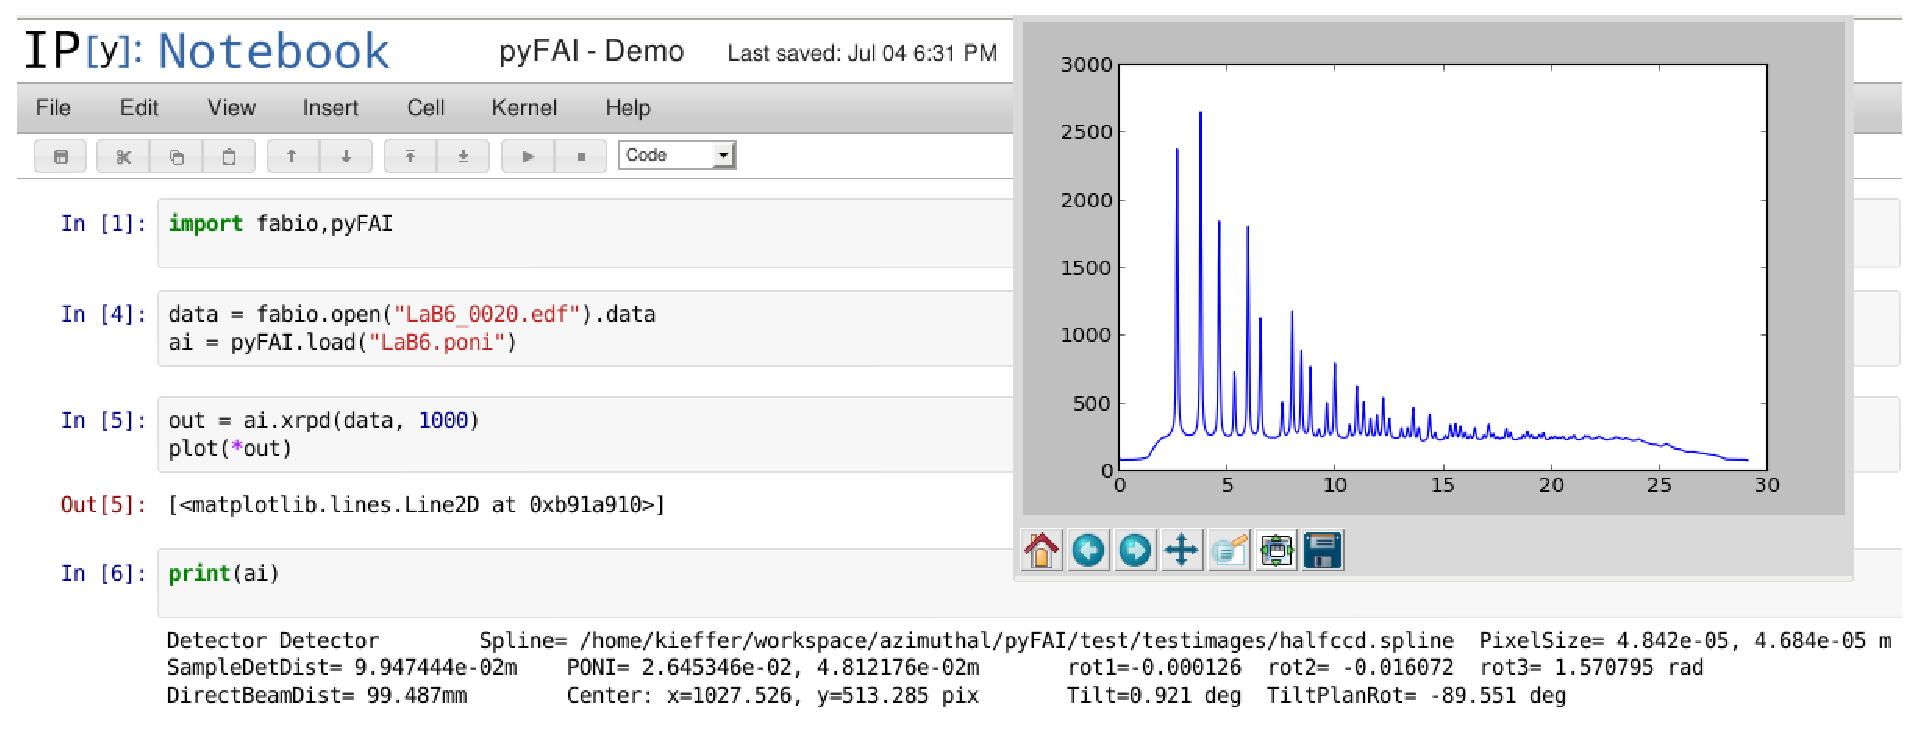
\includegraphics[width=15cm]{img/notebook-l.eps}
\caption{\label{notebook} Example of interactive use of fabio and pyFAI in the
interactive environment ipython.}
\end{figure}
\end{center}
	

\section{Regrouping mechanism} 
Azimuthal-regrouping is done in pyFAI using a histogram-like algorithm: every
pixel of the input image is associated to it's coordinate in polar coordinate
(2q, c) or (q, c) .Then a couple of histograms of 2q (or q) are build: one non 
weighted for measuring the number of pixels falling in each bin and another
weighted by pixel  intensities. The division of the weighted histogram by the
number of  pixels per bin gives the powder pattern.  $2d$ regrouping (caking)  is
obtained in the same way using a two-dimensional histogram over radial and
azimuthal  angles.

\subsection{Pixel splitting algorithm}
Powder diffraction patterns obtained by histogram have a major weakness where
statistic is low: a high level of  noise is observed usually close to the beam
stop and when the typical bin-size  is of the size of a pixel. This is
particularly striking when considering  $2d$-regrouped (but the same phenomenon is
present in  $1d$ as well) where most of the bins close to the beam-stop are not
populated by  any pixel . As we can see on Figure XX most of the area affected
by this is  shaded by the beam-stop, but such a compromise was not acceptable:
the  $2d$-regrouping of a smooth image should be smooth.

\begin{center}
\begin{figure}[h]
\begin{minipage}{8cm}
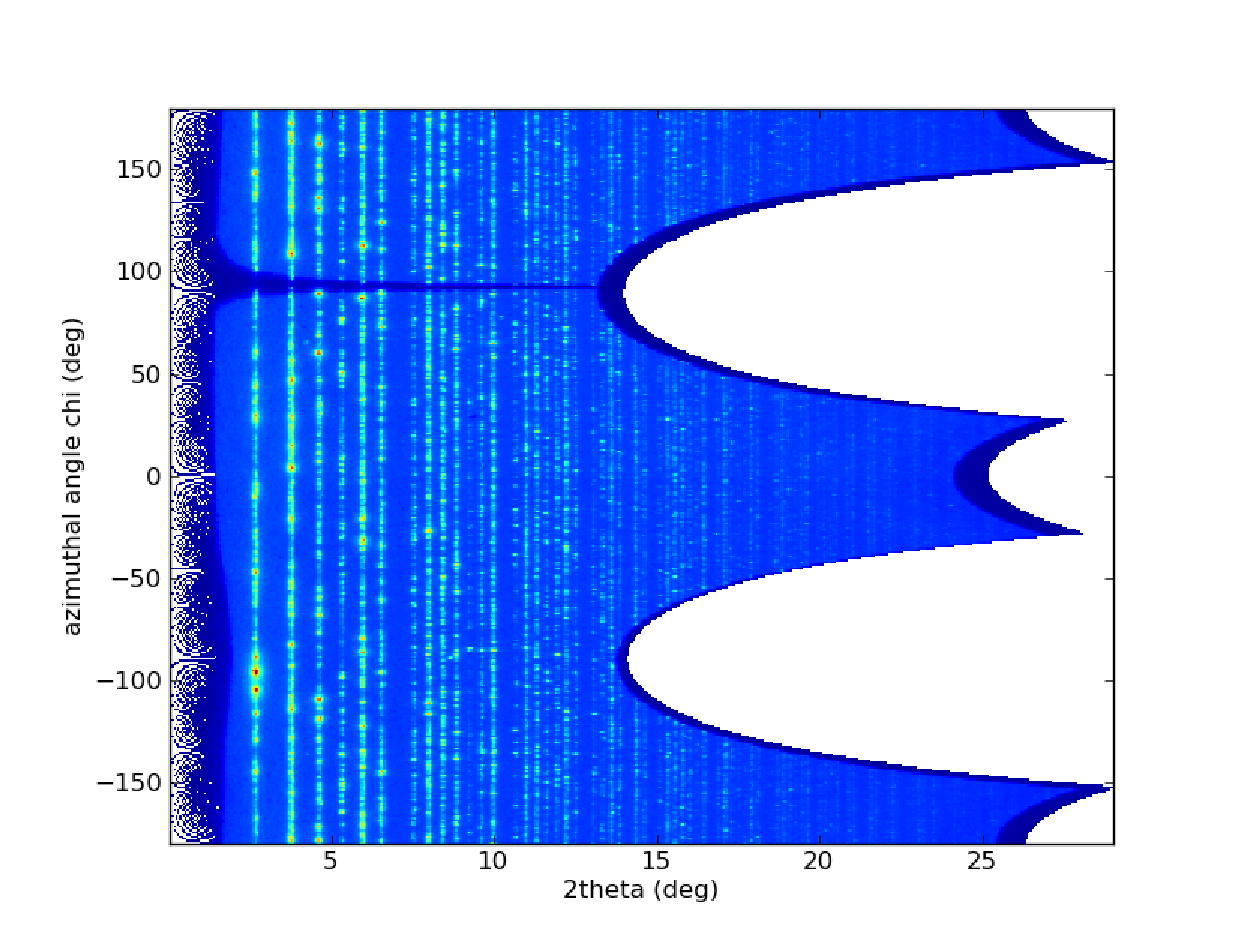
\includegraphics[width=8cm]{img/2Dhistogram.eps}
\caption{\label{rough}$2d$-regrouped image without pixel splitting.}
\end{minipage}\hspace{5mm}
\begin{minipage}{8cm}
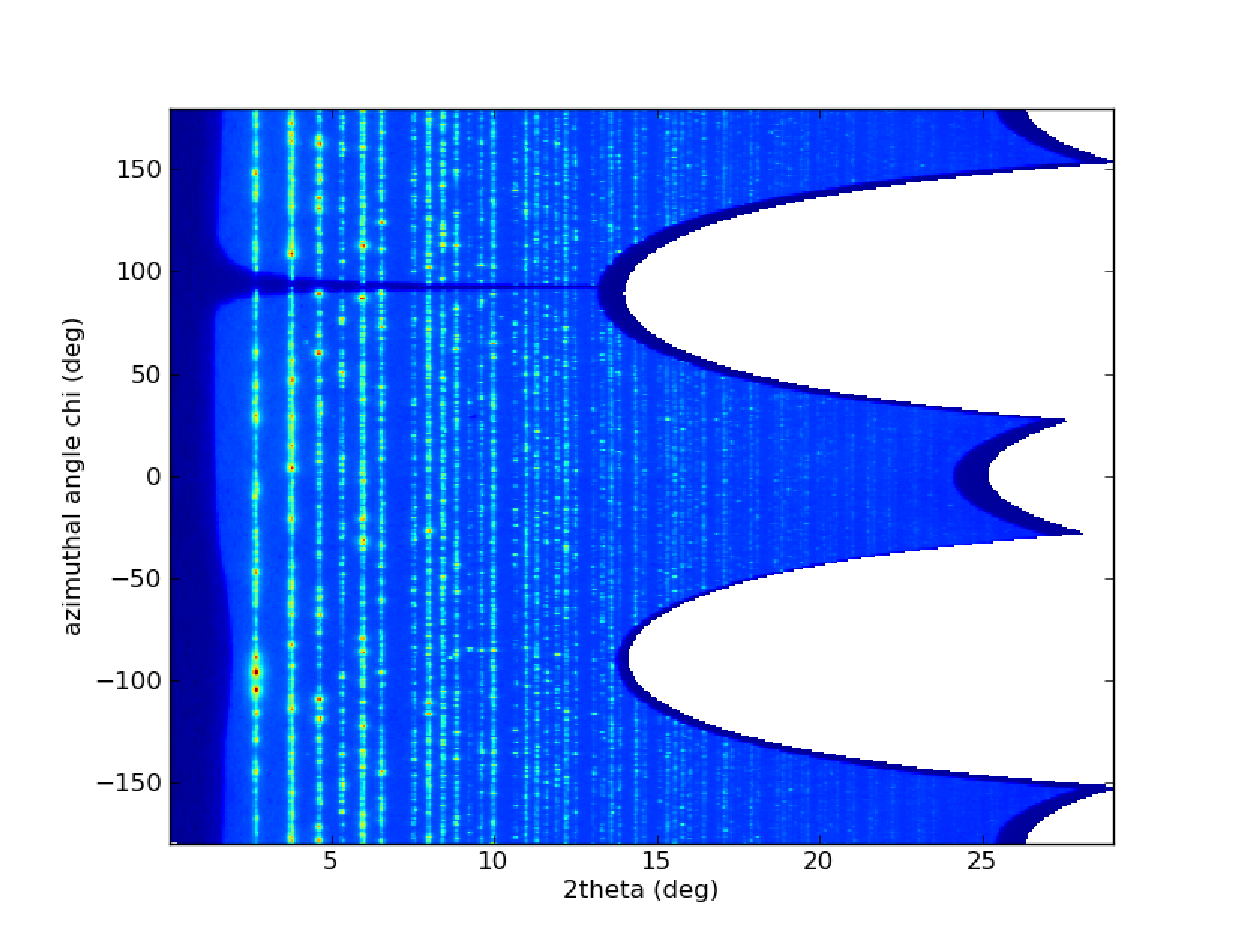
\includegraphics[width=8cm]{img/2DwithSplit.eps}
\caption{\label{smooth}$2d$-regrouped image with pixel splitting.}
\end{minipage} 
\end{figure}
\end{center}

PyFAI solves this problem by considering in addition the spatial extension of
every pixel, both in radial    and azimuthal direction. Every pixel is then splitted and distributed over the corresponding bins. Intensity is assumed to be homogeneous over a single pixel.
\subsection{Performances and migration to native code}
Computation time is proportional to the size of the input image and almost
independent  of the number of bins. Originally the regrouping was implemented 
using the histogram and histogram2d provided by numpy[]. As this step is the
most  time consuming, it was re-implemented and optimized using cython to
achieve  a  3 to 4 times speed-up compared to numpy.
The pixel splitting algorithm was also implemented in cython, enhancing the 
original histogram and optimized to give excellent single-threaded performances 
around 20 Hz/Mpixel.

\subsection{Graphic card implementation}
Graphical Processing Unit (GPU) are composed of hundreds of
small computing cores; they are optimized for highly parallel  algorithms 
whith speed-ups going up to 3 orders of magnitude over sequetial  code running
on Central Processing Unit (CPU).
While histograms do not fall into this category, they can  neverthless be ported
to GPUs efficiently. In order to benefit from GPU acceleration, the Open
Computing Language (OpenCL) was used. OpenCL can make use of multiple  different
devices such as CPUs and GPUs with very different features and capabiities

this
framework also allows the code to utilize multiple CPU cores, which was
useful for validation.


was used ; it allows programming both , a programming languange and
API[footnote] those GPU need also a specific programming languages:

Diffrations images having milions of pixels,
histograms have to be done in double precision with atomic operations whereas
most OpenCL implementations currently only offer simple precision arythmethics.

%The most challanging part is 

\subsection{Performances}
\begin{table}[h]
\caption{\label{blobs}Performances obtained on two Intel XeonX5690 @3.47GHz and various GPU: C2075 and GTX580 are professional and consumer grade Fermi class nVidia GPU with 512 cores.\\
 The table reports execution time measured in miliseconds on various size of images in double precision except for the FireGL v7800\footnote{FireGL v7800 is only capable of single precision atomic operation.}.}
\begin{center}
\begin{tabular}{|l|c||c|c||c|c|c|c|}
\hline
Image               & Image size 	& \multicolumn{2}{|c||}{CPU X5690}& \multicolumn{4}{|c|}{OpenCL $1d$ regrouping} \\
					& mega pixels	& $1d$	&	$2d$	&	X5690	&	C2075	&	GTX580	&	FireGL SP\\
\hline
Pilatus-1M 			&1 	 			& 34.4  &	63.1	&	13.9	&	7.2		&	6.3		&	13.8 \\
Half Frelon 		&2 	 			& 76.6  &   132.4   &	23.4	&	14.4	&	12.2	&	18.8 \\
Frelon 				& 4  			& 165.0	&	269.4   &	52.6	&	34.1	&	28.2	&	40.0 \\
Pilatus-6M 			& 6  			& 232.0	&	350.7	&	74.4	&	49.8	&	40.7	&	48.1 \\
Fairchaild 			& 16 			& 613.9	&	849.7   &	158.9	&	99.0	&	96.4	&	95.6 \\
\hline
\end{tabular}
\end{center}
\end{table}

The OpenCL implementation of pyFAI is very fast on GPU, but less optimized in on
CPU. The profiling of the code revealed other bottlenecks to be addressed in
futur optimisation:
loading data from file, converting arrays of integers to float and transfering this array to the
graphic card. The $2d$ regrouping of powder images will also be integrated in
pyFAI in future releases 

\section{Conclusion}


A library such as pyFAI has two main goals:
\begin{itemize} 
\item Performing azimuthal integration wich
offers a clean interface to developers or scientists in the field of X-ray
diffraction and provide outstanding performances.
\item No compromize on the quality of the result: carreful management of the
geometry, pixel splitting, total and local intensity conservation.
\end{itemize} 

This ten folds speed up in azimuthal integration opens the door to a new
kind of analysis, not even considered until today: a scientist could write
himself a small script of a dozen of lines of code for analysing a diffraction
tomography experiment (typically 60 x 200 frames),  such analysis would only
take a few minutes using pyFAI when it used to take days for data reduction only.
PyFAI is the tool to couple with the next generation hi-speed detectors.

 
\subsection*{Acknowledgments}
Authors wishing to acknowledge assistance or encouragement from 
colleagues, especially Manuel S\'anchez del R\'io for suggesting the usage of
of weighted histograms.
V. Armando Sol\'e for his expertise on developing native under windows, Jonathan
Wright and all the ESRF-ID11 team for the specification and Peter B\"osecke for
the geometry used in pyFAI. Porting pyFAI to GPU would not have been
possible without the financial support of LinkSCEEM-2 (RI-261600).

\subsection*{Appendices}
PyFAI is an open source softare released une the GPL licence. 
As of July 2012, pyFAI is available in version 0.6 on the EPN-Campus forge[]
which includes OpenCL acceleration.
It needs in addition to python v2.6 or v2.7, numpy and OpenCL library.
In order to be able to read images from various detector, pyFAI relies on the
fabio[] library available from sourceforge. The graphical user interface for 
calibration of diffraction setup uses in adition matplotlib, scipy, and FFTw3.
To build pyFAI from source TODO

PyFAI is packaged and available in common Linux distributions like Debian
7.0 and Ubuntu 12.04 (in version 0.3.5). Install packages for Windows are also
available on the EPN-Campus forge.

 \section*{References}
\begin{thebibliography}{9}
\bibitem{iopartnum} IOP Publishing is to grateful Mark A Caprio, Center for Theoretical Physics, Yale University, for permission to include the {\tt iopart-num} \BibTeX package (version 2.0, December 21, 2006) with  this documentation. Updates and new releases of {\tt iopart-num} can be found on \verb"www.ctan.org" (CTAN). 
\end{thebibliography}

\end{document}


